\documentclass[border=6pt]{standalone}
\usepackage[T1]{fontenc}
\usepackage{lmodern}
\usepackage{pgfplots}
\pgfplotsset{compat=1.16}
% Generated by make_cost_figure.py from analysis/cost_model.json. Prediction, not a measurement.
\begin{document}
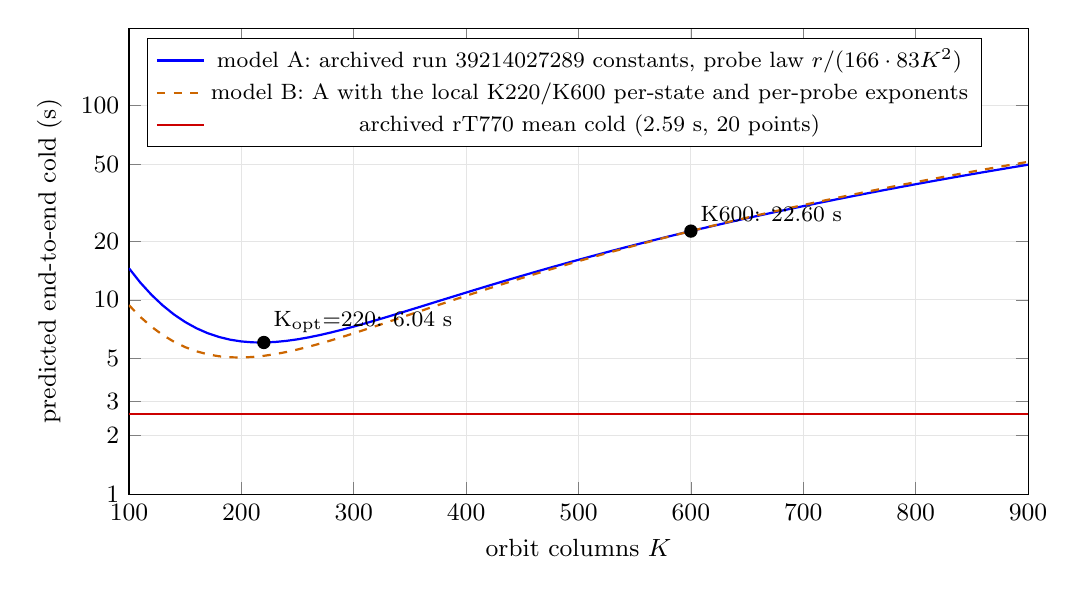
\begin{tikzpicture}
\begin{axis}[width=13cm, height=7.5cm, xlabel={orbit columns $K$}, ylabel={predicted end-to-end cold (s)},
  ymode=log, xmin=100, xmax=900, ymin=1, ymax=250, grid=both, grid style={gray!20},
  ytick={1,2,3,5,10,20,50,100}, log ticks with fixed point,
  legend style={at={(0.02,0.98)}, anchor=north west, font=\footnotesize}, font=\small]
\addplot[thick, blue] coordinates {(100,14.5491) (110,12.2944) (120,10.6238) (130,9.3684) (140,8.4172) (150,7.6949) (160,7.1489) (170,6.7419) (180,6.4464) (190,6.2419) (200,6.1131) (210,6.0481) (220,6.0378) (230,6.0748) (240,6.1534) (250,6.2690) (260,6.4178) (270,6.5966) (280,6.8030) (290,7.0349) (300,7.2904) (310,7.5681) (320,7.8668) (330,8.1853) (340,8.5228) (350,8.8784) (360,9.2515) (370,9.6415) (380,10.0479) (390,10.4703) (400,10.9082) (410,11.3612) (420,11.8292) (430,12.3119) (440,12.8089) (450,13.3201) (460,13.8452) (470,14.3842) (480,14.9369) (490,15.5031) (500,16.0827) (510,16.6756) (520,17.2817) (530,17.9008) (540,18.5331) (550,19.1782) (560,19.8362) (570,20.5071) (580,21.1907) (590,21.8870) (600,22.5959) (610,23.3175) (620,24.0516) (630,24.7983) (640,25.5574) (650,26.3290) (660,27.1131) (670,27.9095) (680,28.7184) (690,29.5396) (700,30.3731) (710,31.2190) (720,32.0771) (730,32.9476) (740,33.8303) (750,34.7252) (760,35.6324) (770,36.5518) (780,37.4834) (790,38.4272) (800,39.3831) (810,40.3513) (820,41.3316) (830,42.3241) (840,43.3287) (850,44.3454) (860,45.3743) (870,46.4153) (880,47.4684) (890,48.5337) (900,49.6110)};
\addlegendentry{model A: archived run 39214027289 constants, probe law $r/(166\cdot 83K^2)$}
\addplot[thick, dashed, orange!80!black] coordinates {(100,9.3913) (110,8.1822) (120,7.2796) (130,6.6013) (140,6.0921) (150,5.7138) (160,5.4393) (170,5.2490) (180,5.1282) (190,5.0659) (200,5.0537) (210,5.0851) (220,5.1547) (230,5.2586) (240,5.3935) (250,5.5566) (260,5.7458) (270,5.9593) (280,6.1955) (290,6.4533) (300,6.7316) (310,7.0294) (320,7.3461) (330,7.6810) (340,8.0335) (350,8.4032) (360,8.7896) (370,9.1925) (380,9.6115) (390,10.0464) (400,10.4968) (410,10.9627) (420,11.4438) (430,11.9400) (440,12.4511) (450,12.9770) (460,13.5177) (470,14.0730) (480,14.6428) (490,15.2271) (500,15.8258) (510,16.4389) (520,17.0663) (530,17.7079) (540,18.3637) (550,19.0338) (560,19.7180) (570,20.4163) (580,21.1287) (590,21.8553) (600,22.5959) (610,23.3506) (620,24.1193) (630,24.9021) (640,25.6990) (650,26.5098) (660,27.3347) (670,28.1736) (680,29.0266) (690,29.8935) (700,30.7745) (710,31.6695) (720,32.5786) (730,33.5016) (740,34.4388) (750,35.3899) (760,36.3551) (770,37.3343) (780,38.3276) (790,39.3350) (800,40.3564) (810,41.3919) (820,42.4414) (830,43.5051) (840,44.5828) (850,45.6747) (860,46.7807) (870,47.9008) (880,49.0350) (890,50.1833) (900,51.3458)};
\addlegendentry{model B: A with the local K220/K600 per-state and per-probe exponents}
\addplot[thick, red!80!black, domain=100:900, samples=2] {2.5939};
\addlegendentry{archived rT770 mean cold (2.59 s, 20 points)}
\addplot[only marks, mark=*, mark size=2.2pt, black] coordinates {(220,6.0378) (600,22.5959)};
\node[anchor=south west, font=\footnotesize] at (axis cs:220,6.0378) {K$_\mathrm{opt}$=220: 6.04 s};
\node[anchor=south west, font=\footnotesize] at (axis cs:600,22.5959) {K600: 22.60 s};
\end{axis}
\end{tikzpicture}
\end{document}
